% Template for Carleton problem sets
% Author: Andrew Gainer-Dewar, 20131
\documentclass[twoside]{article}
\usepackage{ccpset}
\usepackage{graphicx, pdfpages}
\usepackage{fixltx2e}
\usepackage{tabularx}

% The Latin Modern font is a modernized replacement for the classic
% Computer Modern. Feel free to replace this with a different font package.
\usepackage{lmodern}

%\titleformat{\subsection}[runin]{}{}{}{}[]

\title{EE445L - Lab 06 Report}
\author{Kevin Gilbert\\ Gilberto Rodriguez}
\date{March 7 2014}
\prof{Professor Bard}
\course{Lab: Monday/Wednesday 5-6:15}

\begin{document}
\raggedbottom
\maketitle{}

\section*{Requirements Document}
\subsection*{Overview} 
\subsubsection*{Objectives} 
The objectives of this project are to design, build and test a music player. Educationally, students are learning how to interface a DAC, how to design a speaker amplifier, how to store digital music in ROM, and how to perform DAC output in the background. Your goal is to play your favorite song. 
 
\subsubsection*{Process}
The project will be developed using the LM3S1968 board. There will be three switches that the operator will use to control the music player. The system will be built on a solderless breadboard and run on the usual USB power. The system may use the on board switches or off-board switches. A hardware/software interface will be designed that allows software to control the player. There will be at least three hardware/software modules: switch input, DAC output, and the music player. The process will be to design and test each module independently from the other modules. After each module is tested, the system will be built and tested. 
 
\subsubsection*{Roles and Responsibilities}
EE445L students are the engineers and the TA is the client. Students are expected to make minor modifications to this document in order to clarify exactly what they plan to build. Students are allowed to divide responsibilities of the project however they wish, but, at the time of demonstration, both students are expected to understand all aspects of the design. 
 
\subsubsection*{Interactions with Existing Systems}
 The system will use the LM3S1968 board, a solderless breadboard, and the speaker. It will be powered using the USB cable. You may use a +5V power from the lab bench, but please do not power the speaker with a voltage above +5V. 
 
\subsubsection*{Terminology}
 	\begin{enumerate}
    	\item SSI: Synchronous Serial Interface. Communication standard using a shared clock signal, a data signal, and slave select signals.
        \item Linearity: Used in reference to the audio amplifier, linearity determines how the amplifier's output matches to its input. If discrete increments of the input lead to discrete increments in the output of an equal rate of growth at a larger value, then the amplifier has a linear function.
        \item Frequency Response: Measure of the audio amplifier's range of inputs to output spectrum.
        \item Loudness: How loud a tone is. Determined by the amplitude of the output wave, which is in turn determined by the digital value sent to the DAC (larger values provide a higher output voltage).
        \item Pitch: Frequency of a wave.
        \item Instrument: Type of sound being played in this lab. Can be adjusted by outputing a non-sine wave. Controlling the voltage over time plot of the wave can create new instrumental sounds.
        \item Tempo: The speed at which the song is played. Controlled by how often notes are changed.
        \item Envelope: The exponential drop in amplitude of the sound waves over time to provide smoother signals.
        \item Melody: The primary sequence of notes to form a song's core.
        \item Harmony: Accompanying sequence of notes that form a backdrop for a melody.
	\end{enumerate}
 
\subsubsection*{Security} 
The system may include software from StellarisWare and from the book. No software written for this project may be transmitted, viewed, or communicated with any other EE445L student past, present, or future (other than the lab partner of course). It is the responsibility of the team to keep its EE445L lab solutions secure. 
 
\subsection*{Function Description} 
\subsubsection*{Functionality} 
If the operator presses the play/pause button the music will play or pause. If the operator presses the play/pause button once the music should pause. Hitting the play/pause again causes music to continue. The play/pause button does not restart from the beginning, rather it continues from the position it was paused. If the rewind button is pressed, the music stops and the next play operation will start from the beginning. There is a mode Lab 5 Music Player and Audio Amp switch that allows the operator to control the volume of the music player. There must be a C data structure to hold the music. There must be a music driver that plays songs. The length of the song should be at least 30 seconds and comprise of at least 8 different sounds. Although you will be playing only one song, the song data itself will be stored in a separate place and be easy to change. The player runs in the background using interrupts. The foreground (main) initializes the player, then executes for(;;)\{\} do nothing loop. If you wish to include OLED output, this output should occur in the foreground. The maximum time to execute one instance of the ISR is 1.798 $\mu$s. You will need public functions Rewind, Play and Stop, which perform operations like a cassette tape player. The Play function has an input parameter that defines the song to play. A background thread implemented with output compare will fetch data out of your music structure and send them to the DAC. There must be a C data structure to store the sound waveform, or instrument. You are free to design your own format, as long as it uses a formal data structure (i.e., struct). The generated music must sound beautiful utilizing the SNR of the DAC. Although you only have to implement one instrument, it should be easy to change instruments. 
 
\subsubsection*{Scope} 
Phase 1 is the preparation; phase 2 is the demonstration; and phase 3 is the lab report. Details can be found in the lab manual. 
 
\subsubsection*{Prototypes}
A prototype system running on the LM3S1968 board and solderless breadboard will be demonstrated. Progress will be judged by the preparation, demonstration and lab report. 
 
\subsubsection*{Performance} 
The system will be judged by three qualitative measures. First, the software modules must be easy to understand and well-organized. Second, the system must employ an abstract data structures to hold the sound and the music. There should be a clear and obvious translation from sheet music to the data structure. Backward jumps in the ISR are not allowed. Waiting for SSI output to complete is an acceptable backwards jump. Third, all software will be judged according to style guidelines. Software must follow the style described in Section 3.3 of the book. There are three quantitative measures. First, the SNR of the DAC output of a sine wave should be measured. Second, the maximum time to run one instance of the ISR will be recorded. Third, you will measure power supply current to run the system. There is no particular need to optimize any of these quantitative measures in this system.

\subsubsection*{Usability} 
There will be three switch inputs. The DAC will be interfaced to a 8-ohm speaker. 

\subsubsection*{Safety} 
 If you are using headphones, please verify the sound it not too loud before placing the phones next to your ears. 
 
\subsection*{Deliverables} 
\subsubsection*{Reports} 
A lab report described below is due by the due date listed in the syllabus. This report includes the final requirements document. 
 
\subsubsection*{Audits} 
The preparation is due at the beginning of the lab period on the date listed in the syllabus. 
 
\subsubsection*{Outcomes}
There are three deliverables: preparation, demonstration, and report.

\section*{Hardware Design}
\emph{Battery we will use}\\
\centerline{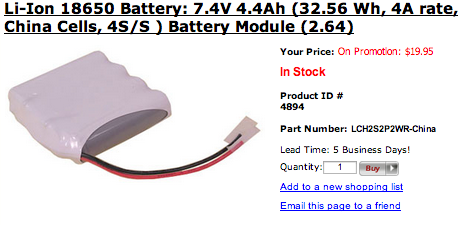
\includegraphics[width=\textwidth]{Battery}}
\centerline{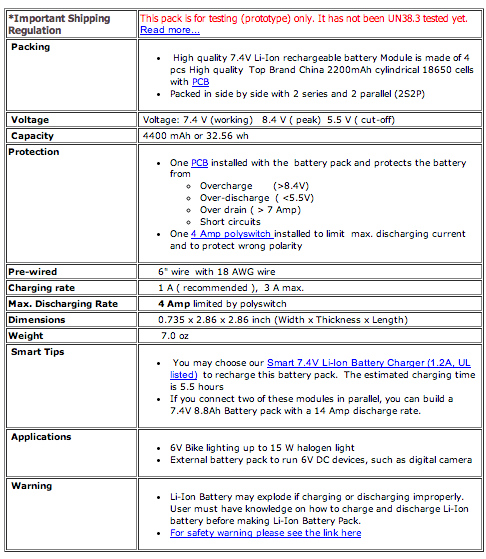
\includegraphics[width=\textwidth]{Battery_Info}}
\emph{Battery info}\\
\centerline{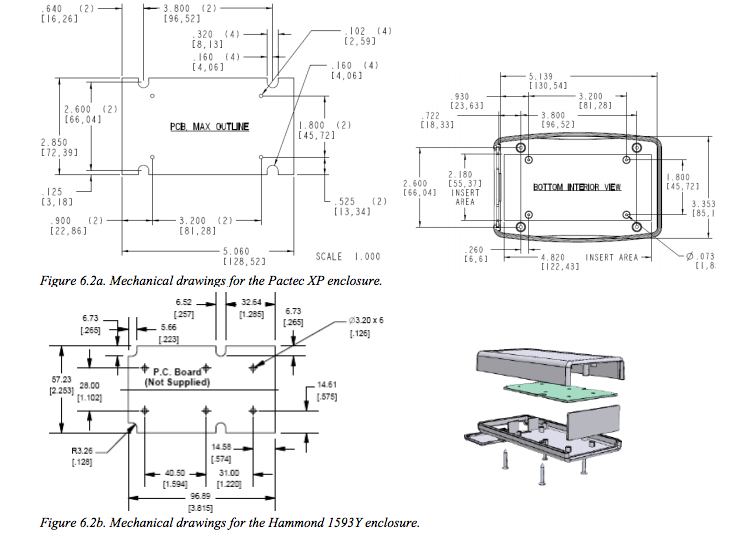
\includegraphics[width=\textwidth]{Box}}
\emph{Used default box}\\
\centerline{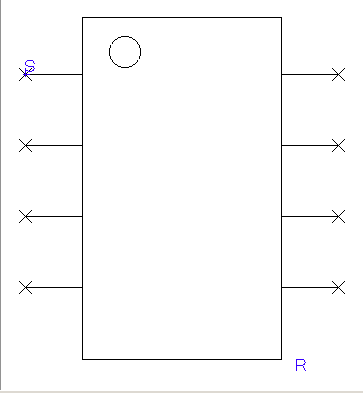
\includegraphics[width=\textwidth]{Foot}}
\emph{Our custom part: TPA301}\\
\centerline{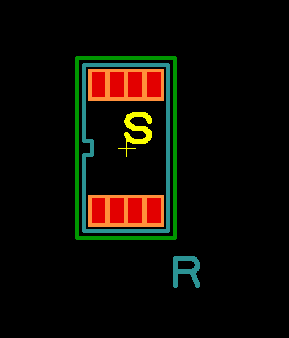
\includegraphics[width=\textwidth]{Foot2}}
\centerline{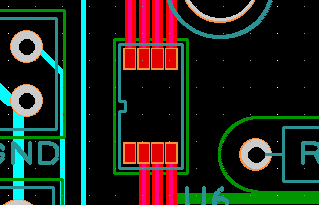
\includegraphics[width=\textwidth]{Foot3}}
 Two mechanical drawings (Procedure 9)\\ 
\centerline{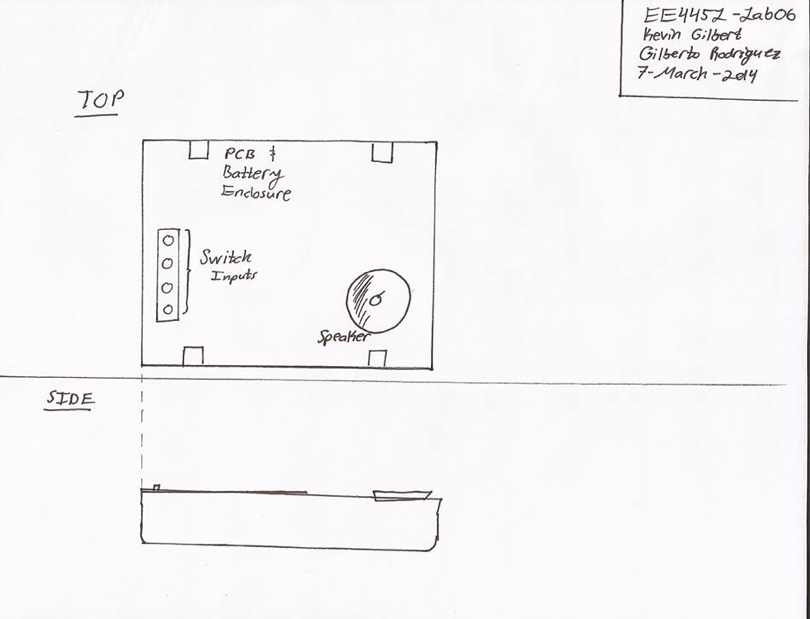
\includegraphics[width=\textwidth]{Lab06_mockup}}
\centerline{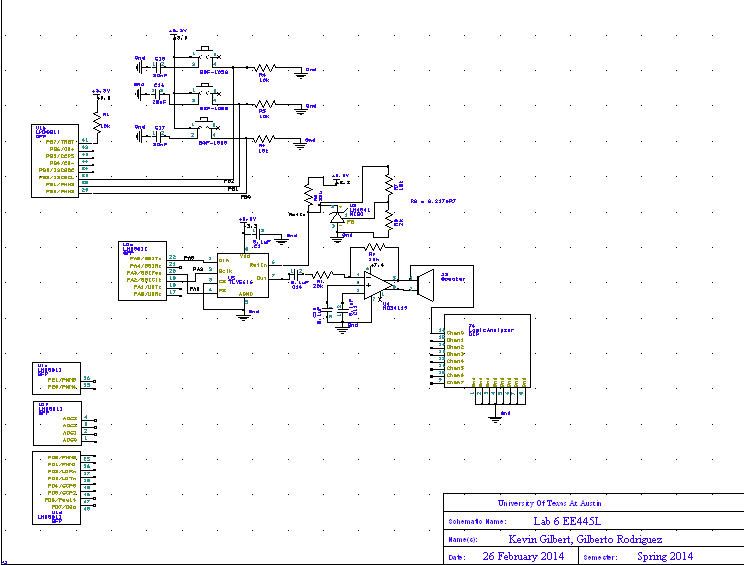
\includegraphics[width=\textwidth]{Circuit}}
\centerline{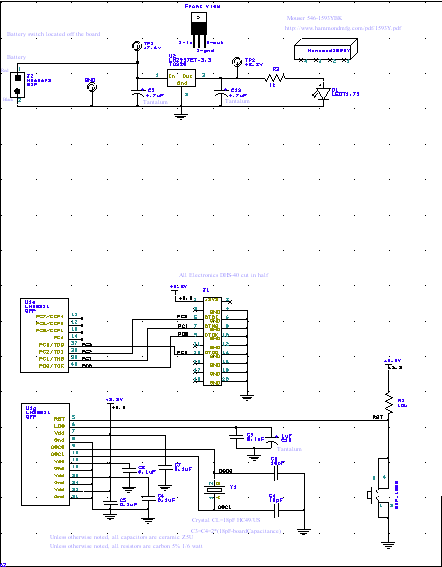
\includegraphics[width=\textwidth]{Circuit2}}
\centerline{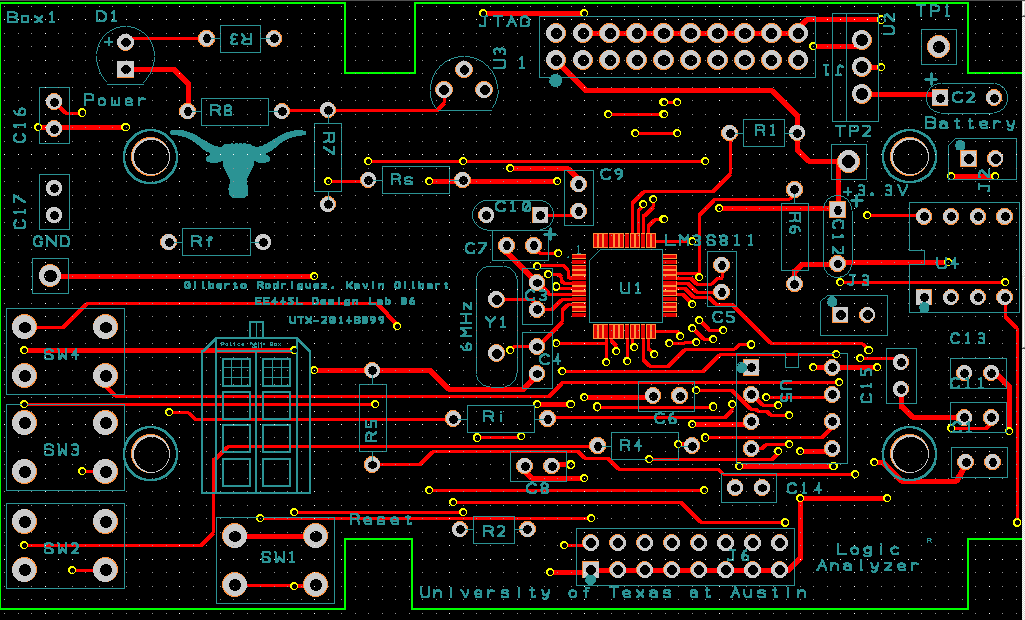
\includegraphics[width=\textwidth]{PCB}}
\vskip 0.1in
\centerline{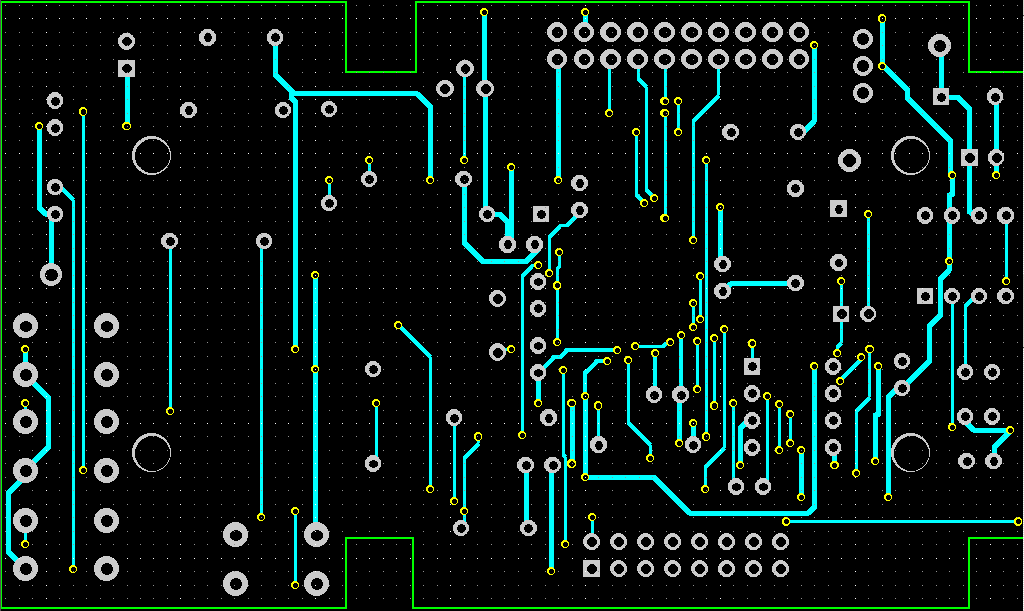
\includegraphics[width=\textwidth]{PCB2}}


\section*{Measurement Data}
\subsection*{Build of Materials}
\begin{center}
  \begin{tabularx}{\textwidth}{ | p{0.10\textwidth} | p{0.1\textwidth} | p{0.10\textwidth} | p{0.15\textwidth} | p{0.16\textwidth} | p{0.23\textwidth} | }
    \hline
    Component & Quantity & Price & Vendor & Current & Information \\ \hline
    Resistor & 5 & \$0.08-1 & Digi-Key & - & 0.25kWatt, 10k$\Omega$ \\ \hline
    Resistor & 2 & \$0.08-1 & Digi-Key & - & 0.12kWatt, 10k$\Omega$ \\ \hline
    Resistor & 4 & \$0.08-1 & Digi-Key & - & 0.25kWatt, 1k$\Omega$(1), 2k$\Omega$(1), 20k$\Omega$(1), 22k$\Omega$(1) \\ \hline
    B3F-1050 & 4 & \$0.29-1 & Mouser & - & Switchs DIP \\ \hline
    Capacitor & 4 & \$0.35-1 & Digi-Key & - & 5\% NonPolar 0.1$\mu$F \\ \hline
    Capacitor & 3 & \$0.35-1 & Digi-Key & - & 5\% NonPolar 20nF \\ \hline
    Capacitor & 7 & \$0.37-1 & Digi-Key & - & 5\% Ceramic  0.1$\mu$F(5),10pF(1),18pF(1) [MCU and Clock Filters]\\ \hline
    Capacitor & 3 & \$0.37-1 & Digi-Key & - & 5\% Polar 1$\mu$F(1), 4.7$\mu$F(2) \\ \hline
    Header2 & 1 & \$2.00-1 & Samtech & - & SIP Power Pins (J2) \\ \hline
    DHS-40 JTAG & 1 & \$2.00-1 & Samtech & - & J1 JTAG Connectors \\ \hline
    LED T1.75 & 1 & \$0.52-1 & Digi-Key & - & LED (D1) \\ \hline
    LM3S811 QFP & 1 & \$6.39-1 & Newark & - & MCU \\ \hline
    LM2937ET-3.3 & 1 & \$0.92-1 - 1kU & TI & 5mA & TO220 (Voltage Regulator U2) \\ \hline
    LM4041 & 1 & \$0.29-1 & Digi-Key & - & Shunt Voltage Reference (U3) \\ \hline
    Pins & 1 & \$2.00-1 & Samtech & - & Logic Analyzer Headers DIP (J6) \\ \hline
    Hammond-1593Y & 1 & \$4.82-1 & Mouser & - & Box (Box1) \\ \hline
    MC34119 & 1 & \$0.50-1 & Digi-Key & - & Audio Amplifier DIP (U4) \\ \hline
    TLV5616 & 1 & \$4.08-1 & Digi-Key & - & DAC DIP (U5) \\ \hline
    Clock-XTAL & 1 & \$1.60 & Digi-Key & - & DSC Y1 \\ \hline   
    Battery & 1 & \$19.85-1 & Batter Space & - & 7.4V Li-Ion Battery \\ \hline
  \end{tabularx}
\end{center}

Bill of Materials (quantity, package type, cost, and supply current) (Procedure 2) \\
Our music player uses a current of 145mA, so we chose a battery that could power the music play for 24 hours while it is running. The battery we chose has a capacity of 4400mAh, which can power our music player for approximately 30 hours.\\


\section*{Analysis and Discussion}
Using the onboard JTAG pins, we would flash code to test the capabilities of each device through a set of testing points. To make the process stream-lined, these testing points would have traces connected to a set of logic analyzer pins. These pins can be monitered during an automated testing procedure to verify the operation of the device. Specically, speaker output is measured in our current design; however, additional test points at the DAC output, DAC inputs, button inputs, and audio amplifier connections could be tested as well. Specifically, a 8-pin digital analyzer attached to these points would allow for observing the response of the system. The software component would generate several sine waves of varying frequencies\\

\end{document}